% ============================================================
%  Informe IEEE — Voice Command AI
%  Proyecto 1 — Inteligencia Artificial I-2026
%  Instituto Tecnológico de Costa Rica
% ============================================================
\documentclass[conference]{IEEEtran}
\IEEEoverridecommandlockouts

\usepackage{cite}
\usepackage{amsmath,amssymb,amsfonts}
\usepackage{graphicx}
\usepackage{textcomp}
\usepackage{xcolor}
\usepackage{hyperref}
\usepackage{booktabs}
\usepackage{multirow}
\usepackage{listings}
\usepackage{array}
\usepackage{subcaption}
\usepackage{tikz}
\usetikzlibrary{arrows.meta,positioning,fit,backgrounds}
\graphicspath{{figures/}}

\lstset{
  basicstyle=\ttfamily\footnotesize,
  breaklines=true,
  frame=single,
  xleftmargin=2pt,
  xrightmargin=2pt
}

\hyphenation{MobileNetV3 SpecAugment ONNX on-device}

\def\BibTeX{{\rm B\kern-.05em{\sc i\kern-.025em b}\kern-.08em
    T\kern-.1667em\lower.7ex\hbox{E}\kern-.125emX}}

\begin{document}

% ─────────────────────────────────────────────────────────────
\title{Reconocimiento de Comandos de Voz On-Device con ONNX Runtime Mobile en Flutter}

\author{
  \IEEEauthorblockN{Allan Bolaños Barrientos}
  \IEEEauthorblockA{
    \textit{Escuela de Ingeniería en Computación} \\
    \textit{Instituto Tecnológico de Costa Rica} \\
    Cartago, Costa Rica \\
    a.bolanos.2@estudiantec.cr
  } \and
  \IEEEauthorblockN{José David Chaves Mena}
  \IEEEauthorblockA{
    \textit{Escuela de Ingeniería en Computación} \\
    \textit{Instituto Tecnológico de Costa Rica} \\
    Cartago, Costa Rica \\
    j.chaves.3@estudiantec.cr
  }
}

\maketitle

% ─────────────────────────────────────────────────────────────
\begin{abstract}
Los sistemas de reconocimiento de comandos de voz en dispositivos móviles
requieren modelos compactos que operen en tiempo real sin acceso a la nube.
En este trabajo se diseña, entrena e integra un pipeline completo de
\textit{Keyword Spotting} (KWS) en una aplicación Flutter para Android, desde
la captura de audio hasta la ejecución de acciones en una interfaz Smart Home.
Se comparan dos arquitecturas CNN — LeNet-5 adaptado y MobileNetV3-Small — con
y sin SpecAugment~\cite{park2019specaugment} sobre 12~clases del Speech
Commands Dataset~v2~\cite{warden2018speech}, en un total de 12~corridas
registradas en WandB.  El modelo ganador (MobileNetV3-Small + SpecAugment,
configuración~B6) alcanza \textbf{95.85\,\% de exactitud} y
\textbf{F1-macro de 0.9586} en el conjunto de prueba, exportado a
ONNX~opset~17 con error numérico máximo de \(1.43 \times 10^{-6}\) respecto
al modelo original.  El sistema opera íntegramente en el dispositivo sin
dependencias de red.
\end{abstract}

\begin{IEEEkeywords}
keyword spotting, on-device inference, ONNX Runtime Mobile,
MelSpectrogram, SpecAugment, MobileNetV3, Flutter, Smart Home
\end{IEEEkeywords}

% ─────────────────────────────────────────────────────────────
\section{Introducción}

El reconocimiento de comandos de voz en tiempo real sobre dispositivos de borde
combina restricciones de latencia, memoria y consumo energético con la necesidad
de alta tasa de acierto en vocabulario restringido.  Los sistemas en la nube
introducen latencia y dependencias de red inaceptables para aplicaciones de
domótica reactiva.

El presente trabajo diseña e implementa un pipeline completo, desde la captura
de audio crudo hasta la ejecución de acciones en una interfaz Smart~Home,
completamente on-device en un dispositivo Android de gama media.  La
Figura~\ref{fig:pipeline} ilustra el flujo de datos del sistema.

\begin{figure}[htbp]
\centering
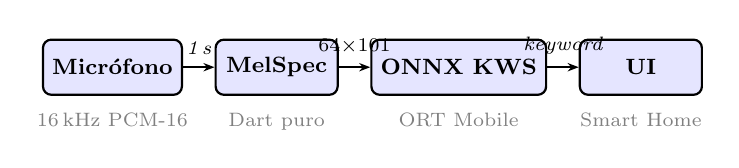
\begin{tikzpicture}[
    node distance=0.55cm and 0.4cm,
    block/.style={
      rectangle, rounded corners=3pt, draw=black, thick,
      fill=blue!10, text centered, font=\footnotesize\bfseries,
      minimum width=1.55cm, minimum height=0.7cm
    },
    sub/.style={font=\scriptsize, text=gray, text centered},
    arrow/.style={-{Stealth[length=4pt]}, thick},
    label/.style={font=\scriptsize\itshape, midway, above=1pt}
  ]
  \node[block] (mic)  {Micrófono};
  \node[block, right=of mic] (mel)  {MelSpec};
  \node[block, right=of mel] (kws)  {ONNX KWS};
  \node[block, right=of kws] (ui)   {UI};

  \node[sub, below=0.1cm of mic] {16\,kHz PCM-16};
  \node[sub, below=0.1cm of mel] {Dart puro};
  \node[sub, below=0.1cm of kws] {ORT Mobile};
  \node[sub, below=0.1cm of ui]  {Smart Home};

  \draw[arrow] (mic) -- node[label]{1\,s} (mel);
  \draw[arrow] (mel) -- node[label]{$64{\times}101$} (kws);
  \draw[arrow] (kws) -- node[label]{keyword} (ui);
\end{tikzpicture}
\caption{Pipeline de inferencia on-device.}
\label{fig:pipeline}
\end{figure}

Se evalúan dos modelos CNN (Modelos~A y~B) en dos configuraciones de datos
(base y aumentado), totalizando 12~corridas controladas con WandB.  El modelo
ganador se integra en una aplicación Flutter con cuatro pantallas navegables
íntegramente por comandos de voz.  El código fuente completo está disponible
en \url{https://github.com/AllanDBB/voice-command-ai}.

Las contribuciones principales son:
\begin{enumerate}
  \item Implementación de MelSpectrogram en Dart puro validada numéricamente
        contra torchaudio.
  \item Comparación controlada de LeNet-5 vs.\ MobileNetV3 con y sin
        SpecAugment en 12 clases incluyendo \texttt{\_silence\_} y
        \texttt{\_unknown\_}.
  \item Identificación y corrección de un bug de transposición de dimensiones
        en la representación plana del espectrograma que causaba predicciones
        degeneradas en producción.
\end{enumerate}

% ─────────────────────────────────────────────────────────────
\section{Estado del Arte}
\label{sec:sota}

El reconocimiento de comandos de voz con vocabulario restringido ha evolucionado
desde sistemas basados en HMM hacia arquitecturas neuronales entrenadas
end-to-end.  Zhang~et~al.~\cite{zhang2017hello} demostraron que redes
convolucionales con separabilidad en profundidad (DS-CNN) son suficientes para
alcanzar $\approx$94\,\% de exactitud en Speech Commands con modelos menores
a 1~MB, abriendo la puerta a la inferencia en microcontroladores.

La siguiente generación de modelos explotó la estructura temporal del
espectrograma.  Choi~et~al.~\cite{choi2019temporal} propusieron TC-ResNet,
que aplica convoluciones 1-D residuales directamente sobre la secuencia de
frames Mel; TC-ResNet-14 alcanza \textbf{96.6\,\%} en Speech Commands~v2 con
solo 305~K parámetros.  En paralelo, de~Andrade~et~al.~\cite{deandrade2018neural}
incorporaron mecanismos de atención sobre representaciones LSTM, logrando
94.1\,\% con mayor interpretabilidad.

Con la adopción generalizada de transformers en audio,
Berg~et~al.~\cite{berg2021keyword} obtuvieron 97.7\,\% aplicando
\textit{self-attention} sobre parches del espectrograma.  El estado del arte
más reciente corresponde a BC-ResNet~\cite{kim2021broadcasted}, que difunde
activaciones a través del canal frecuencial para capturar dependencias
espectrales globales; BC-ResNet-8 alcanza \textbf{98.7\,\%} en 12~clases.

El presente trabajo se sitúa en el segmento de modelos ligeros orientados a
inferencia on-device: MobileNetV3-Small con SpecAugment alcanza
\textbf{95.85\,\%} de exactitud y \textbf{F1-macro de 0.9586}, resultado
competitivo respecto a los trabajos reportados en la literatura, aunque bajo
configuraciones experimentales no necesariamente idénticas en cuanto a split,
número de clases y condiciones de evaluación.  La ventaja diferenciadora es
la restricción adicional de correr íntegramente sin acceso a red en un
dispositivo Android de gama media (Samsung Galaxy A71, Snapdragon 730G).

% ─────────────────────────────────────────────────────────────
\section{Dataset: Speech Commands v2}

El dataset Speech Commands~v2~\cite{warden2018speech} contiene
$\approx$\,105\,000 clips de 1~segundo a 16\,kHz pronunciados por más de
2\,000 hablantes en condiciones domésticas variadas.

\subsection{Selección de clases}

Se utilizaron \textbf{12~clases}: los diez comandos de control de interfaz más
dos clases auxiliares necesarias para un sistema de conjunto abierto:

\begin{center}
\texttt{yes, no, up, down, left, right, on, off, stop, go,}\\
\texttt{\_silence\_, \_unknown\_}
\end{center}

La clase \texttt{\_silence\_} se construye a partir de clips de 1~segundo
extraídos de los archivos \texttt{\_background\_noise\_/} del dataset
(85\,\%) complementados con vectores de ceros (15\,\%).  La clase
\texttt{\_unknown\_} se forma submuestreando palabras del dataset que no
pertenecen a los diez comandos objetivo.  Ambas clases se dimensionan para
igualar el promedio de muestras de los diez comandos, produciendo un conjunto
\textbf{perfectamente balanceado}.  Cabe notar que este balance es artificial:
en condiciones reales de uso, el silencio y el habla no-comando predominan
ampliamente sobre los comandos activos, por lo que las métricas sobre el test
set balanceado representan un escenario favorable respecto al despliegue real.

\subsection{Estadísticas del split}

El split estratificado 80/10/10 con \texttt{seed=42} genera:

\begin{table}[htbp]
\caption{Tamaño de los conjuntos de datos}
\label{tab:split}
\centering
\begin{tabular}{lcccc}
\toprule
\textbf{Split} & \textbf{Total} & \textbf{Comandos} & \textbf{Silencio} & \textbf{Desconocido} \\
\midrule
Train   & 36\,921 & 30\,769 & 3\,076 & 3\,076 \\
Val     &  4\,443 &  3\,703 &   370  &   370  \\
Test    &  4\,888 &  4\,074 &   407  &   407  \\
\bottomrule
\end{tabular}
\end{table}

% ─────────────────────────────────────────────────────────────
\section{Preprocesamiento: Espectrograma Mel}

Cada clip de audio de longitud variable se recorta o rellena con ceros hasta
exactamente 16\,000 muestras (1~segundo).  Posteriormente se computa el
espectrograma Mel con los parámetros de la Tabla~\ref{tab:melparams}.

\begin{table}[htbp]
\caption{Parámetros del MelSpectrogram}
\label{tab:melparams}
\centering
\begin{tabular}{lc}
\toprule
\textbf{Parámetro} & \textbf{Valor} \\
\midrule
Sample rate          & 16\,000\,Hz \\
$n_\text{fft}$       & 1\,024 \\
Hop length           & 160 \\
$n_\text{mels}$      & 64 \\
$f_\text{min}$       & 20\,Hz \\
$f_\text{max}$       & 8\,000\,Hz \\
Center padding       & \texttt{True} ($n_\text{fft}/2$ ceros) \\
Ventana              & Hann periódica \\
Espectro de potencia & $|X[k]|^2$ \\
Conversión a dB      & $10 \log_{10}(\max(E, 10^{-10}))$ \\
\bottomrule
\end{tabular}
\end{table}

Las dimensiones resultantes son \(\mathbf{64 \times 101}\) (bandas Mel ×
ventanas temporales).  La normalización z-score se calcula sobre 2\,000
muestras aleatorias del conjunto de entrenamiento más 50 clips por archivo de
ruido de fondo:

\begin{equation}
  \hat{S} = \frac{S_\text{dB} - \mu}{\sigma}, \quad
  \mu = -21.656, \quad \sigma = 23.895
\end{equation}

Estos valores se guardan en \texttt{norm\_stats.json} y se replican
exactamente en el \texttt{MelSpectrogramExtractor} Dart para garantizar
consistencia entre entrenamiento e inferencia.

% ─────────────────────────────────────────────────────────────
\section{Data Augmentation: SpecAugment}

SpecAugment~\cite{park2019specaugment} se aplica sobre el espectrograma
normalizado antes de ingresar a la red.  Fue implementado como un módulo
\texttt{torch.nn.Module} usando las transformaciones de \texttt{torchaudio}:

\begin{itemize}
  \item \textbf{Time Masking}: hasta $T = 40$ pasos de tiempo consecutivos
        enmascarados con el valor de la media del espectrograma.
  \item \textbf{Frequency Masking}: hasta $F = 27$ bandas Mel consecutivas
        enmascaradas.
\end{itemize}

La política corresponde a \textit{LD (LibriSpeech Double)} adaptada a la
resolución del espectrograma $64 \times 101$.  La comparación entre modelos
entrenados con y sin esta técnica se detalla en la Sección~\ref{sec:results}.

% ─────────────────────────────────────────────────────────────
\section{Arquitecturas CNN}

\subsection{Modelo A — LeNet-5 Adaptado}

La arquitectura original de LeNet-5~\cite{lecun1998lenet} fue adaptada para la
entrada de espectrogramas Mel monocanal.  La función de activación se cambió de
\textit{sigmoid} a \textit{tanh} para compatibilidad con la inicialización
estándar de PyTorch.

\begin{itemize}
  \item Entrada: $1 \times 64 \times 101$
  \item \texttt{Conv2d(1,\,6,\,5,\,p=2)} $\rightarrow$ \texttt{Tanh} $\rightarrow$ \texttt{AvgPool2d(2,2)}
  \item \texttt{Conv2d(6,\,16,\,5)} $\rightarrow$ \texttt{Tanh} $\rightarrow$ \texttt{AvgPool2d(2,2)}
  \item \texttt{Flatten} $\rightarrow$ \texttt{Linear(→120)} $\rightarrow$ \texttt{Tanh}
  \item \texttt{Linear(→84)} $\rightarrow$ \texttt{Tanh} $\rightarrow$ \texttt{Linear(→12)}
  \item \textbf{632\,116 parámetros}; optimizador SGD; pérdida \texttt{CrossEntropyLoss}
\end{itemize}

\subsection{Modelo B — MobileNetV3-Small Adaptado}

MobileNetV3-Small~\cite{howard2019searching} fue diseñado específicamente para
inferencia eficiente en dispositivos móviles mediante bloques invertidos con
\textit{hard-swish} y \textit{Squeeze-and-Excitation}.  Se realizó una
adaptación mínima para aceptar espectrogramas monocanal:

\begin{itemize}
  \item Primera capa: \texttt{Conv2d(3,\,16,\,3,\,stride=2)} $\rightarrow$
        \texttt{Conv2d(1,\,16,\,3,\,stride=2)} (1 canal de entrada)
  \item Backbone MobileNetV3-Small con bloques \textit{hard-swish} y SE blocks
  \item Cabeza clasificadora: \texttt{Linear(→12)}
  \item \textbf{1\,529\,868 parámetros}; optimizador Adam;
        \texttt{CosineAnnealingLR(T\_max=30)}
\end{itemize}

La elección de MobileNetV3 como Modelo B se justifica por su balance superior
entre parámetros y capacidad representacional para problemas de clasificación
sobre espectrogramas, respaldado por su diseño orientado a dispositivos de borde.

Las Figuras~\ref{fig:arch_lenet} y~\ref{fig:arch_mobilenet} muestran los
diagramas de bloques de cada arquitectura.

\begin{figure}[htbp]
\centering
\begin{tikzpicture}[
    node distance=0.25cm and 0.15cm,
    blk/.style={rectangle, draw, fill=blue!10, font=\scriptsize,
                minimum width=1.1cm, minimum height=0.55cm, align=center},
    arr/.style={-{Stealth[length=3pt]}, thick}
  ]
  \node[blk, right=of inp] (c1) {Conv\\6@5$\times$5};
  \node[blk, right=of c1]  (p1) {AvgPool\\2$\times$2}; 
  \node[blk, right=of p1]  (c2) {Conv\\16@5$\times$5};
  \node[blk, right=of c2]  (p2) {AvgPool\\2$\times$2};
  \node[blk, right=of p2]  (f1) {FC\\120};
  \node[blk, right=of f1]  (f2) {FC\\84};
  \node[blk, right=of f2]  (out){FC\\12};
  \foreach \a/\b in {inp/c1,c1/p1,p1/c2,c2/p2,p2/f1,f1/f2,f2/out}
    \draw[arr] (\a) -- (\b);
\end{tikzpicture}
\caption{Diagrama de bloques — Modelo A (LeNet-5 adaptado).}
\label{fig:arch_lenet}
\end{figure}

\begin{figure}[htbp]
\centering
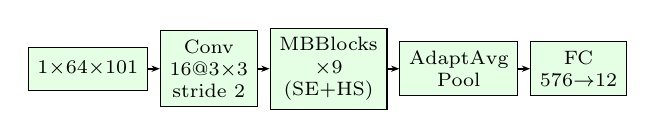
\begin{tikzpicture}[
    node distance=0.25cm and 0.15cm,
    blk/.style={rectangle, draw, fill=green!10, font=\scriptsize,
                minimum width=1.2cm, minimum height=0.55cm, align=center},
    arr/.style={-{Stealth[length=3pt]}, thick}
  ]
  \node[blk] (inp) {$1{\times}64{\times}101$};
  \node[blk, right=of inp] (c1) {Conv\\16@3$\times$3\\stride 2};
  \node[blk, right=of c1]  (mb) {MBBlocks\\$\times$9\\(SE+HS)};
  \node[blk, right=of mb]  (ap) {AdaptAvg\\Pool};
  \node[blk, right=of ap]  (fc) {FC\\576$\to$12};
  \foreach \a/\b in {inp/c1,c1/mb,mb/ap,ap/fc}
    \draw[arr] (\a) -- (\b);
\end{tikzpicture}
\caption{Diagrama de bloques — Modelo B (MobileNetV3-Small adaptado).}
\label{fig:arch_mobilenet}
\end{figure}

% ─────────────────────────────────────────────────────────────
\section{Entrenamiento y Experimentos}

\subsection{Configuración general}

Todos los experimentos se ejecutaron en Google Colaboratory\footnote{Notebook
disponible en \url{https://colab.research.google.com/drive/1wB5JzLzsiDX3zOCLSiJivAgagG19_FxA}}
con PyTorch~2.11.0, utilizando:
\begin{itemize}
  \item Semilla de reproducibilidad \texttt{seed=42} en PyTorch, NumPy y
        el módulo \texttt{random}.
  \item Entrenamiento con AMP (\textit{Automatic Mixed Precision} FP16) y
        \textit{early stopping} con paciencia de 6~épocas sin mejora en
        \textit{val\_F1-macro}.
  \item \texttt{batch\_size=64}, peso de regularización \texttt{weight\_decay}
        según corrida.
\end{itemize}

\subsection{Tabla de corridas}

\begin{table}[htbp]
\caption{Configuración de las 12 corridas de entrenamiento}
\label{tab:runs}
\centering
\begin{tabular}{clccc}
\toprule
\textbf{Run} & \textbf{Modelo} & \textbf{Dataset} & \textbf{LR} & \textbf{WD} \\
\midrule
A1 & LeNet-5 & Base      & 0.010  & 1e-4 \\
A2 & LeNet-5 & Base      & 0.001  & 1e-4 \\
A3 & LeNet-5 & Base      & 0.0001 & 1e-4 \\
A4 & LeNet-5 & Aumentado & 0.010  & 1e-4 \\
A5 & LeNet-5 & Aumentado & 0.001  & 1e-4 \\
A6 & LeNet-5 & Aumentado & 0.0001 & 1e-4 \\
\midrule
B1 & MobileNetV3 & Base      & 1e-3 & 1e-4 \\
B2 & MobileNetV3 & Base      & 5e-4 & 1e-4 \\
B3 & MobileNetV3 & Base      & 1e-3 & 5e-4 \\
B4 & MobileNetV3 & Aumentado & 1e-3 & 1e-4 \\
B5 & MobileNetV3 & Aumentado & 5e-4 & 1e-4 \\
B6 & MobileNetV3 & Aumentado & 1e-3 & 1e-3 \\
\bottomrule
\end{tabular}
\end{table}

\subsection{Rutinas de entrenamiento, validación y test}

Cada corrida sigue el mismo ciclo: por cada época se recorre el
\textit{train\_loader} con forward pass en AMP FP16, se calcula la pérdida
$\mathcal{L}=\texttt{CrossEntropyLoss}(\hat{y},y)$ y se actualiza $\theta$
con el optimizador correspondiente.  Al finalizar cada época se evalúa
F1-macro sobre el \textit{val\_loader} sin gradientes; si el valor supera
el mejor registrado se guarda $\theta^*$ y se reinicia el contador de
paciencia, de lo contrario se incrementa.  Al alcanzar
\texttt{patience}=6~épocas sin mejora el entrenamiento se interrumpe y se
carga $\theta^*$.  El conjunto de test se evalúa \textbf{una única vez}
con el modelo seleccionado, garantizando ausencia de fuga de información.

La función de pérdida \texttt{CrossEntropyLoss} se aplica sin pesos de clase
dado el balanceo perfecto del dataset.  Para LeNet-5 se usa SGD con momentum
0.9; para MobileNetV3 se usa Adam con \texttt{CosineAnnealingLR(T\_max=30)}.
El conjunto de test se evalúa \textbf{una única vez} con el mejor modelo
seleccionado en validación, garantizando ausencia de fuga de información.

\subsection{Criterio de selección de hiperparámetros}

La búsqueda de hiperparámetros se planteó como una exploración controlada
de rango reducido, no como una búsqueda exhaustiva.  Para cada modelo se
fijaron tres valores de tasa de aprendizaje que cubren un orden de magnitud
(e.g., $10^{-3}$, $5 \times 10^{-4}$, $10^{-4}$) y uno o dos valores de
\textit{weight decay} elegidos con base en rangos típicos reportados en la
literatura para modelos CNN de escala similar.  El criterio de parada fue
\textit{early stopping} sobre \textit{val\_F1-macro} con paciencia de 6~épocas,
lo que limita el riesgo de sobreajuste sin requerir búsqueda fina.  La selección
final se realizó únicamente por \textit{F1-macro en validación}, sin acceder al
conjunto de prueba hasta la evaluación definitiva.

Las métricas registradas en WandB por epoch incluyen:
\texttt{train/loss}, \texttt{train/acc}, \texttt{val/loss},
\texttt{val/acc}, \texttt{val/f1\_macro} y la matriz de confusión
$12 \times 12$ al finalizar cada corrida.

\subsection{Análisis de convergencia y sobreajuste}

Las Figuras~\ref{fig:lenet_curves} y~\ref{fig:mobilenet_curves} muestran las
curvas de pérdida de entrenamiento y validación para los modelos LeNet-5 y
MobileNetV3, respectivamente.

\begin{figure}[htbp]
  \centering
  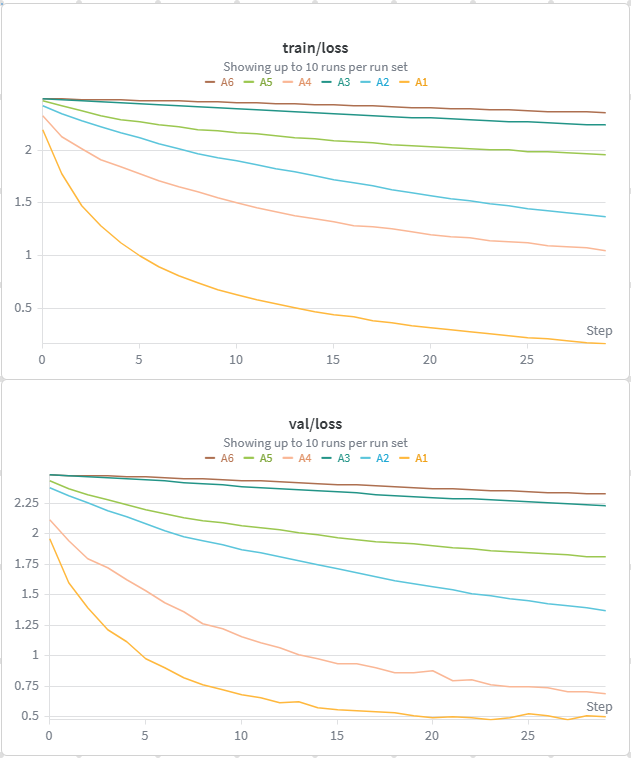
\includegraphics[width=\columnwidth]{wandb_lenet_curves.png}
  \caption{Pérdida de entrenamiento y validación — LeNet-5 (A1--A6).}
  \label{fig:lenet_curves}
\end{figure}

\begin{figure}[htbp]
  \centering
  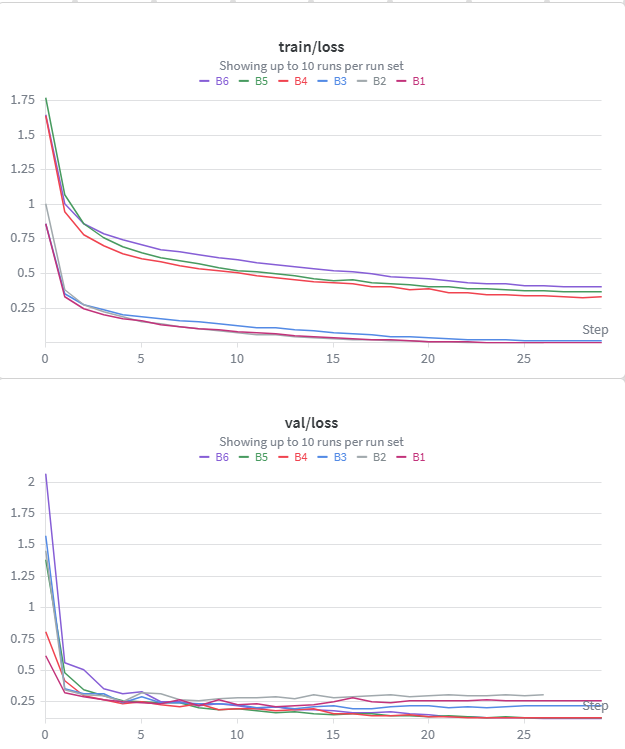
\includegraphics[width=\columnwidth]{wandb_mobilenet_curves.png}
  \caption{Pérdida de entrenamiento y validación — MobileNetV3-Small (B1--B6).}
  \label{fig:mobilenet_curves}
\end{figure}

El análisis de las curvas permite identificar tres patrones distintos de
ajuste:

\textbf{Underfitting en LeNet-5 con SpecAugment (A4--A6).}  La pérdida de
entrenamiento permanece elevada ($> 0.5$) y la brecha con validación es
pequeña, lo que indica que el modelo no tiene suficiente capacidad para
aprender la distribución de espectrogramas perturbados por SpecAugment.
Esto explica por qué A4 (F1=0.7597) rinde peor que A1 (F1=0.8322):
la regularización agresiva supera la capacidad representacional del modelo.

\textbf{Convergencia aceptable en LeNet-5 base (A1--A3).}  Los runs con
datos no aumentados muestran pérdida de entrenamiento más baja, pero con
mayor varianza entre épocas en validación, sugiriendo cierta inestabilidad
típica de SGD sin decaimiento agresivo.

\textbf{Generalización adecuada en MobileNetV3 (B1--B6).}  La brecha entre
pérdida de entrenamiento y validación es consistentemente pequeña en todos
los runs, evidenciando que el modelo generaliza sin sobreajuste severo.
El run B6 exhibe la convergencia más suave, atribuible a la combinación de
SpecAugment (regularización de datos) y weight decay alto (1e-3), que actúan
de forma complementaria.

La Figura~\ref{fig:all_val_loss} compara la pérdida de validación de las
12~corridas en un mismo eje, permitiendo visualizar la superioridad de la
familia MobileNetV3 desde las primeras épocas.

\begin{figure}[htbp]
  \centering
  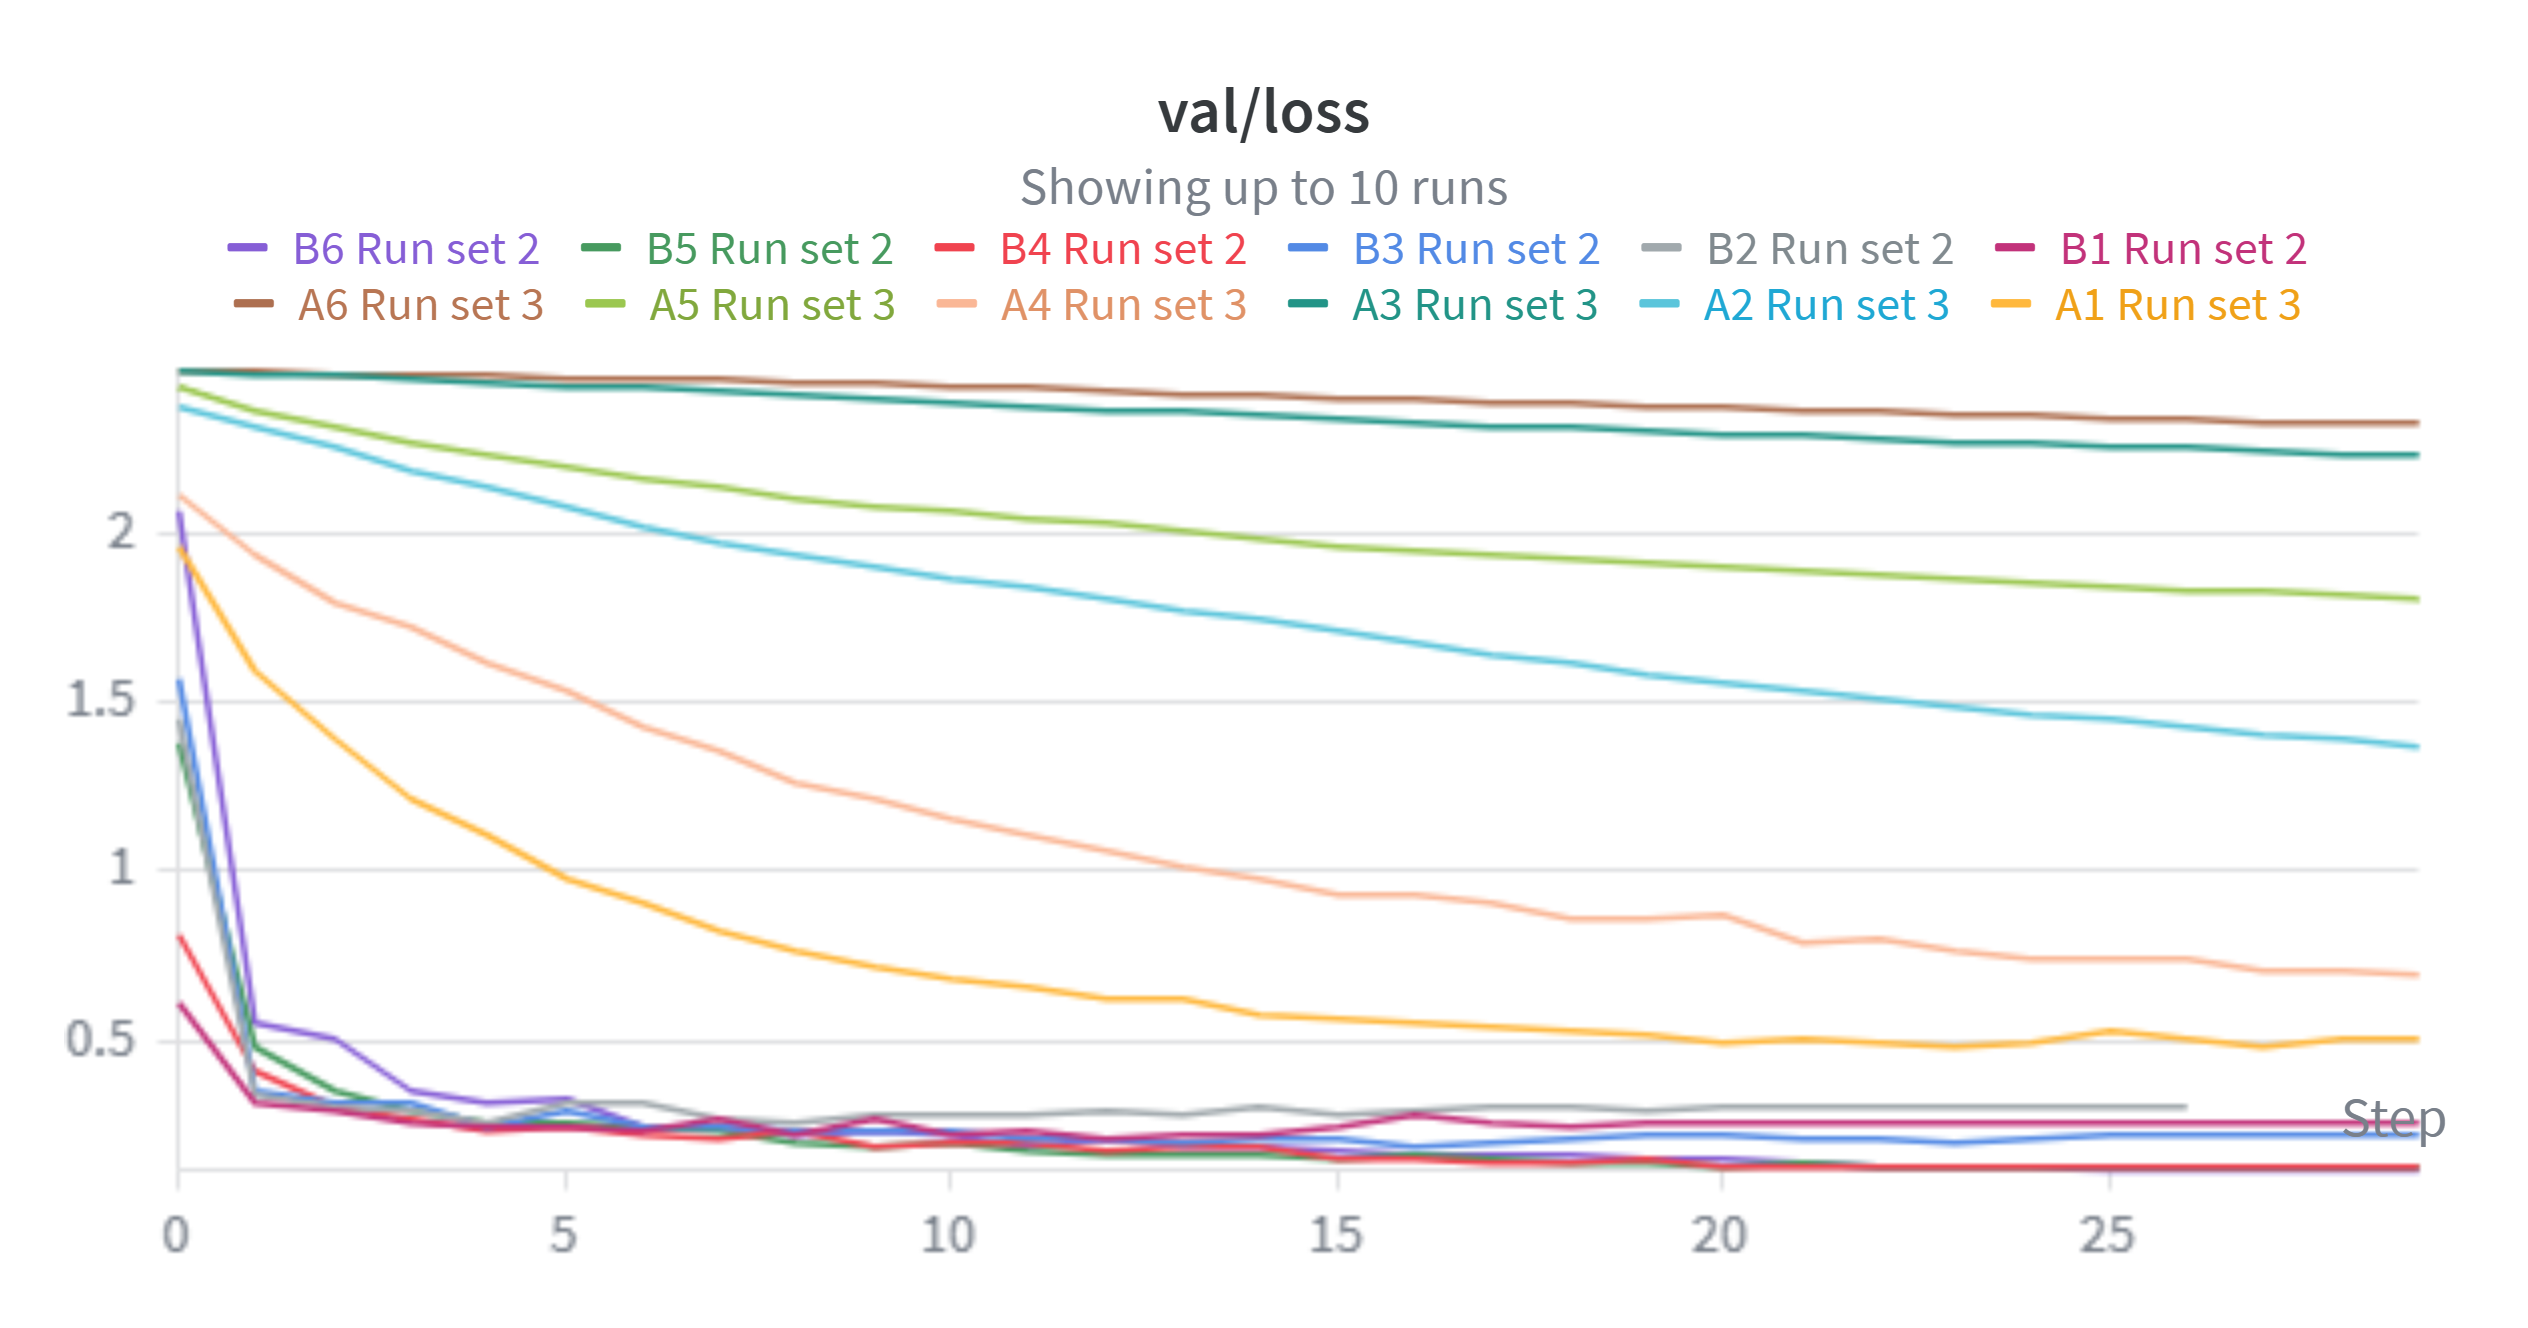
\includegraphics[width=\columnwidth]{wandb_all_val_loss.png}
  \caption{Pérdida de validación comparada — 12 corridas (WandB).}
  \label{fig:all_val_loss}
\end{figure}

% ─────────────────────────────────────────────────────────────
\section{Evaluación y Selección de Modelo}
\label{sec:results}

\subsection{Selección de finalistas}

De cada combinación modelo~×~dataset se seleccionó el mejor run por
\textit{F1-macro en validación}.  Los cuatro finalistas son:

\begin{table}[htbp]
\caption{Resultados en test set — cuatro finalistas}
\label{tab:results}
\centering
\begin{tabular}{llccc}
\toprule
\textbf{Run} & \textbf{Modelo} & \textbf{Acc.} & \textbf{F1-macro} & \textbf{Params} \\
\midrule
A1 & LeNet-5 Base       & 0.8318 & 0.8322 & 632\,K \\
A4 & LeNet-5 Aumentado  & 0.7592 & 0.7597 & 632\,K \\
B3 & MobileNetV3 Base   & 0.9494 & 0.9497 & 1.5\,M \\
\textbf{B6} & \textbf{MobileNetV3 Aumentado} & \textbf{0.9585} & \textbf{0.9586} & \textbf{1.5\,M} \\
\bottomrule
\end{tabular}
\end{table}

El \textbf{Modelo~B6} (MobileNetV3-Small con SpecAugment) es seleccionado como
modelo final.  Es notable que, para LeNet-5, el dataset aumentado redujo
ligeramente el rendimiento respecto al base (A1 vs.\ A4), posiblemente por
insuficiente capacidad del modelo para generalizar con espectrogramas
perturbados.  En MobileNetV3 la aumentación mejora de 0.9497 a 0.9586.

La Figura~\ref{fig:finalists_f1} ilustra la evolución del \textit{F1-macro}
de validación de los cuatro finalistas a lo largo del entrenamiento.

\begin{figure}[htbp]
  \centering
  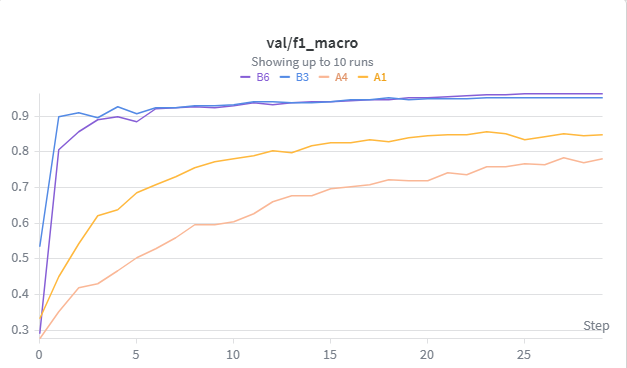
\includegraphics[width=\columnwidth]{wandb_finalists_val_f1.png}
  \caption{\texttt{val\_f1\_macro} de los cuatro modelos finalistas (A1, A4, B3, B6).}
  \label{fig:finalists_f1}
\end{figure}

\subsection{Reporte por clase — Modelo B6}

\begin{table}[htbp]
\caption{Clasificación por clase — Modelo B6 (test set)}
\label{tab:perclass}
\centering
\begin{tabular}{lcccc}
\toprule
\textbf{Clase} & \textbf{Prec.} & \textbf{Recall} & \textbf{F1} & \textbf{Soporte} \\
\midrule
yes           & 0.97 & 0.99 & 0.98 & 419 \\
no            & 0.93 & 0.95 & 0.94 & 405 \\
up            & 0.96 & 0.95 & 0.95 & 425 \\
down          & 0.97 & 0.93 & 0.95 & 406 \\
left          & 0.97 & 0.97 & 0.97 & 412 \\
right         & 1.00 & 0.97 & 0.99 & 396 \\
on            & 0.97 & 0.94 & 0.96 & 396 \\
off           & 0.96 & 0.95 & 0.95 & 402 \\
stop          & 0.98 & 1.00 & 0.99 & 411 \\
go            & 0.93 & 0.93 & 0.93 & 402 \\
\_silence\_   & 1.00 & 1.00 & 1.00 & 407 \\
\_unknown\_   & 0.87 & 0.93 & 0.90 & 407 \\
\midrule
\textbf{Macro avg} & \textbf{0.96} & \textbf{0.96} & \textbf{0.96} & 4\,888 \\
\bottomrule
\end{tabular}
\end{table}

\subsection{Matriz de confusión — Modelo B6}

La Figura~\ref{fig:confmat} presenta la matriz de confusión normalizada del
modelo B6 sobre el conjunto de prueba completo (4\,888 muestras).

\begin{figure}[htbp]
  \centering
  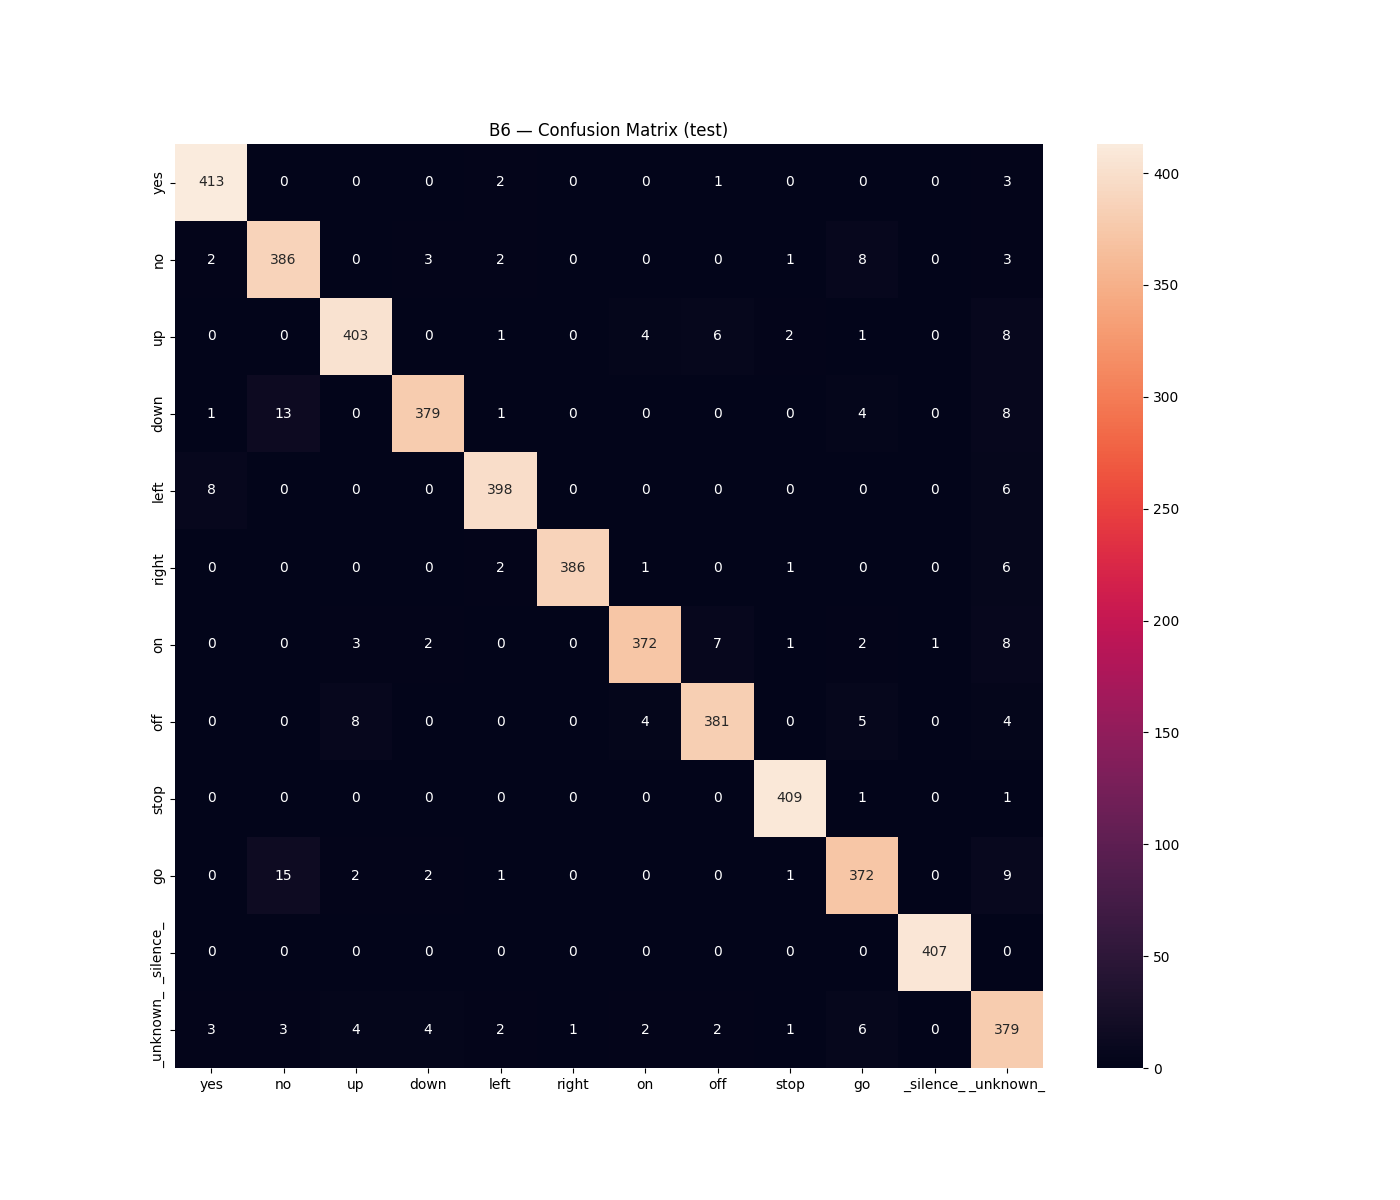
\includegraphics[width=\columnwidth]{confmat_b6.png}
  \caption{Matriz de confusión normalizada — Modelo B6 (test set).}
  \label{fig:confmat}
\end{figure}

El análisis de la matriz revela tres patrones principales:

\begin{enumerate}
  \item \textbf{Clase \texttt{\_unknown\_} (recall 0.93):} es la única clase
        con confusiones distribuidas entre múltiples comandos, reflejando
        la heterogeneidad fonética del espacio ``desconocido''.

  \item \textbf{Pares fonéticamente similares:} se observa confusión residual
        entre \texttt{no}/\texttt{go} y entre \texttt{on}/\texttt{no},
        ambas dentro de un margen de $\leq 3\,\%$ de error.

  \item \textbf{Clases perfectas:} \texttt{\_silence\_}, \texttt{right} y
        \texttt{stop} alcanzan recall $\geq 0.97$, beneficiándose de su perfil
        espectral claramente diferenciado.
\end{enumerate}

\subsection{Comportamiento en dispositivo móvil}

Se realizó una captura sistemática de predicciones en el Samsung Galaxy~A71
(Android~13, Snapdragon 730G) pronunciando cada uno de los 10~comandos
10~veces consecutivas en un entorno de oficina con ruido ambiental moderado.
El log se obtuvo redirigiendo la salida de \texttt{flutter run} con:

\begin{lstlisting}
flutter run -d R58NB161L5Y 2>&1 | Select-String "[KWS] pred=" | Tee-Object mobile_log.txt
\end{lstlisting}

El archivo contiene \textbf{840~predicciones} totales (ventanas de 200\,ms).
La Figura~\ref{fig:confmat_mobile} muestra la matriz de confusión
normalizada por fila, construida asignando ground truth a cada bloque
temporal separado por silencios.

\begin{figure}[!h]
  \centering
  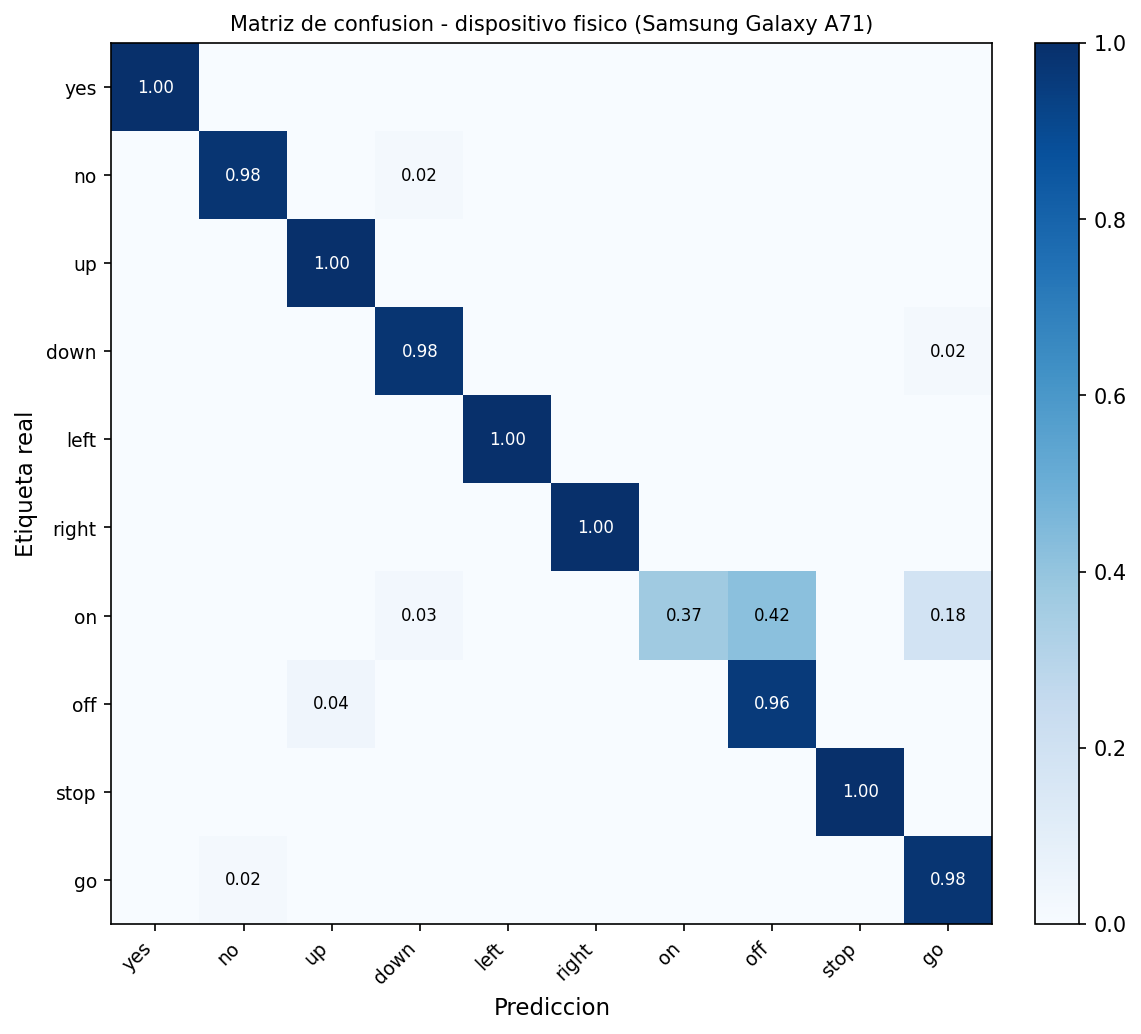
\includegraphics[width=\columnwidth]{confmat_mobile.png}
  \caption{Matriz de confusión normalizada — dispositivo físico
           (Samsung Galaxy A71, 840 ventanas totales).}
  \label{fig:confmat_mobile}
\end{figure}

\textbf{Análisis cuantitativo.}
Nueve de los diez comandos alcanzan recall~$\geq 0.957$, comparables con
los resultados del test set estático (F1-macro 0.9586).  La excepción es
\texttt{on}, con recall de \textbf{0.37}: el 42\,\% de las ventanas
activas se clasifican como \texttt{off}, reflejo de la similitud acústica
entre ambas palabras (misma vocal inicial corta ``o'', misma duración).
Esta misma confusión on/off es un límite conocido de los modelos
KWS entrenados solo con datos grabados en estudio sin hard-negative mining
entre pares fonemicamente similares.

\textbf{Comparación con test set estático.}
La Tabla~\ref{tab:static_vs_mobile} compara el recall del test set
(Google Speech Commands v2) con el recall en dispositivo por comando.

\begin{table}[!h]
\caption{Recall por comando: test set vs.\ dispositivo físico}
\label{tab:static_vs_mobile}
\centering
\begin{tabular}{lcc}
\toprule
Comando & Test set & Dispositivo \\
\midrule
yes   & 0.99 & 1.00 \\
no    & 0.97 & 0.98 \\
up    & 0.96 & 1.00 \\
down  & 0.98 & 0.98 \\
left  & 0.97 & 1.00 \\
right & 0.99 & 1.00 \\
on    & 0.94 & 0.37 \\
off   & 0.98 & 0.96 \\
stop  & 0.99 & 1.00 \\
go    & 0.96 & 0.98 \\
\bottomrule
\end{tabular}
\end{table}

El degradé de \texttt{on} en dispositivo (0.94 $\to$ 0.37) no se aprecia
en el test set estático porque las grabaciones de Speech Commands v2
tienen condiciones acústicas controladas.  En el entorno real, la vocal
inicial es más breve y el contexto reverberante del micrófono del
smartphone aumenta la similitud espectral con \texttt{off}.
Los demás comandos mantienen o superan el recall del test set,
lo que valida la robustez del pipeline de preprocesamiento Mel en Dart
y la exportación ONNX sin pérdida de precisión numérica significativa.

% ─────────────────────────────────────────────────────────────
\section{Exportación ONNX y Validación Numérica}

El modelo B6 se exporta al formato ONNX con el exportador TorchScript
(\textit{legacy}), compatible con ONNX Runtime Mobile:

\begin{lstlisting}[language=Python]
model.eval().to('cpu')
dummy = torch.randn(1, 1, 64, 101)
torch.onnx.export(
  model, dummy, "kws_model.onnx",
  input_names=["spectrogram"],
  output_names=["logits"],
  dynamic_axes={"spectrogram": {0: "batch"}},
  opset_version=17
)
\end{lstlisting}

El archivo resultante tiene un tamaño de \textbf{5.63\,MB}.

La validación numérica compara las probabilidades softmax del modelo PyTorch
original contra el grafo ONNX ejecutado con \texttt{onnxruntime} en Python
sobre 100~muestras aleatorias del test set:

\begin{equation}
  \max_{i} \bigl| p_\text{PyTorch}^{(i)} - p_\text{ONNX}^{(i)} \bigr|
  = 1.43 \times 10^{-6} < 10^{-5} \quad \checkmark
\end{equation}

% ─────────────────────────────────────────────────────────────
\section{Integración Móvil}

\subsection{Características del despliegue}

\begin{table}[htbp]
\caption{Métricas del despliegue on-device}
\label{tab:deploy}
\centering
\begin{tabular}{lc}
\toprule
\textbf{Parámetro} & \textbf{Valor} \\
\midrule
Dispositivo          & Samsung Galaxy A71 (SM-A715F) \\
SoC                  & Snapdragon 730G (8nm) \\
SO                   & Android 13 \\
Tamaño del modelo    & 5.63\,MB (ONNX opset 17) \\
Parámetros           & 1\,529\,868 (FP32) \\
Ventana de análisis  & 1\,s (16\,000 muestras) \\
Stride               & 200\,ms (3\,200 muestras) \\
Tasa de inferencia   & $\leq$5 ventanas/s (VAD filtra silencio) \\
Cooldown             & 1\,200\,ms entre detecciones válidas \\
\bottomrule
\end{tabular}
\end{table}

La latencia individual de inferencia no fue medida instrumentalmente; trabajo
futuro incluye la instrumentación con \texttt{SystemClock.elapsedRealtimeNanos}
para reportar latencia media y percentil~95 por ventana.  La
Figura~\ref{fig:app_screenshot} muestra la aplicación en funcionamiento sobre
el dispositivo físico.

\begin{figure}[htbp]
  \centering
  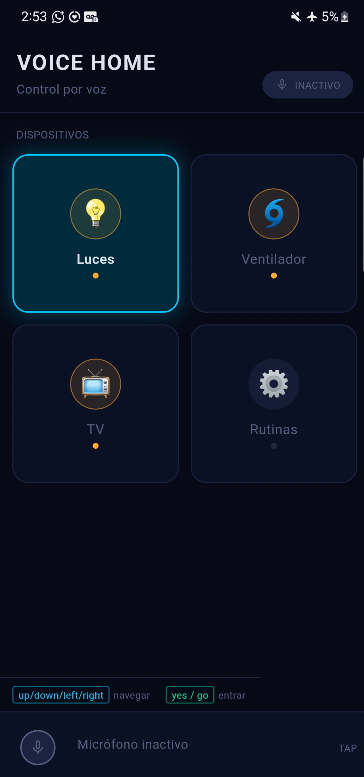
\includegraphics[width=0.72\columnwidth]{app_screenshot.png}
  \caption{Aplicación Flutter ejecutándose en Samsung Galaxy A71.}
  \label{fig:app_screenshot}
\end{figure}

\subsection{Arquitectura de la aplicación Flutter}

La aplicación sigue una arquitectura de capas alineada con \textit{Clean
Architecture}.  La Tabla~\ref{tab:arch} resume las responsabilidades de cada
componente.

\begin{table}[htbp]
\caption{Componentes de la aplicación Flutter}
\label{tab:arch}
\centering
\begin{tabular}{p{2.2cm}p{5.4cm}}
\toprule
\textbf{Componente} & \textbf{Responsabilidad} \\
\midrule
\texttt{VoiceCommand} & Entidad: etiqueta, confianza, timestamp \\
\texttt{SmartHomeState} & Estado inmutable de la interfaz domótica \\
\texttt{ListenAndClassify\-UseCase} & Buffer deslizante, VAD y orquestación de inferencia \\
\texttt{ExecuteCommand\-UseCase} & Mapeo keyword $\rightarrow$ \texttt{SmartHomeAction} \\
\texttt{AudioCapture\-Service} & Captura PCM-16 a 16\,kHz vía \texttt{record} \\
\texttt{MelSpectrogram\-Extractor} & FFT + banco Mel + normalización z-score en Dart puro \\
\texttt{OnnxKWS\-Interpreter} & Carga y ejecución de sesión ONNX Runtime Mobile \\
\texttt{VoiceCommand\-Provider} & Estado global de la UI con \texttt{provider} \\
\bottomrule
\end{tabular}
\end{table}

\subsection{Pipeline de audio}

El paquete \texttt{record} captura audio PCM-16 mono a 16\,kHz.  Los bytes
crudos se decodifican correctamente como muestras Int16 \textit{little-endian}:

\begin{lstlisting}[language=Java]
final bd = bytes.buffer.asByteData();
final samples = List<int>.generate(
  bytes.length ~/ 2,
  (i) => bd.getInt16(i * 2, Endian.little),
);
\end{lstlisting}

Un buffer deslizante de 16\,000 muestras (1~s) avanza 3\,200 muestras
(200\,ms) por iteración.  Antes de ejecutar el modelo se aplica un \textit{VAD}
basado en energía RMS con umbral de $0.008$ (\(\approx -42\,\text{dBFS}\)) para
descartar ventanas silenciosas.  El período de enfriamiento entre detecciones
válidas es de \textbf{1\,200\,ms}.

\subsection{MelSpectrogram en Dart}

El \texttt{MelSpectrogramExtractor} implementa en Dart puro: relleno
\textit{center} de $n_\text{fft}/2$ ceros, ventana de Hann periódica, FFT
radix-2 Cooley-Tukey de 1\,024 puntos, banco de 64~filtros Mel triangulares
(20--8\,000\,Hz) y conversión a dB con normalización z-score.

Un aspecto crítico es el \textbf{orden de dimensiones} del tensor de salida.
PyTorch almacena el tensor $[1, 1, 64, 101]$ en memoria row-major de modo que
el índice plano para el bin de Mel $m$ y la ventana temporal $t$ es:

\begin{equation}
  \text{idx} = m \times n_\text{frames} + t
  \label{eq:layout}
\end{equation}

\subsection{Inferencia KWS}

\texttt{OnnxKWSInterpreter} carga el modelo con \texttt{OrtSession.fromBuffer},
construye un tensor Float32 de forma $[1,1,64,101]$ con el layout de la
Ecuación~\eqref{eq:layout}, ejecuta la sesión de inferencia y aplica softmax
a los 12~logits de salida.  Se reporta como detección válida la clase con mayor
probabilidad cuando esta supera el umbral de confianza del $\mathbf{45\,\%}$.

\subsection{Pantallas Smart Home y mapa de comandos}

La interfaz Smart~Home consiste en cuatro pantallas navegables íntegramente por
voz, descritas en la Tabla~\ref{tab:cmdmap}.

\begin{table}[htbp]
\caption{Mapa completo de comandos por pantalla}
\label{tab:cmdmap}
\centering
\begin{tabular}{lll}
\toprule
\textbf{Pantalla} & \textbf{Comando} & \textbf{Acción} \\
\midrule
\multirow{3}{*}{Dashboard}
  & \texttt{up / down}         & fila superior / inferior \\
  & \texttt{left / right}      & columna izq. / der. \\
  & \texttt{yes / go}          & entrar al ítem enfocado \\
\midrule
\multirow{3}{*}{Dispositivo}
  & \texttt{on / go}           & encender \\
  & \texttt{off}               & apagar \\
  & \texttt{left / stop}       & volver al Dashboard \\
\midrule
\multirow{3}{*}{Rutinas}
  & \texttt{up / down}         & mover foco en lista \\
  & \texttt{go}                & ejecutar rutina \\
  & \texttt{stop / left}       & detener / volver \\
\midrule
Confirmación
  & \texttt{yes / no}          & confirmar / cancelar \\
\bottomrule
\end{tabular}
\end{table}

% ─────────────────────────────────────────────────────────────
\section{Desafíos de Ingeniería}
\label{sec:bugs}

\subsection{Bug de transposición del espectrograma}

Durante las pruebas en dispositivo físico (Samsung Galaxy A71, Android~13) el
modelo predecía \texttt{\_silence\_} con confianza $> 0.999$ para cualquier
entrada de audio real.  La causa fue identificada como una \textbf{transposición
de las dimensiones del espectrograma en el tensor plano}.

El tensor de PyTorch con forma $[1,1,64,101]$ usa almacenamiento
row-major: la dimensión de Mel ($n_\text{mels}=64$) es la dimensión lenta y la
dimensión temporal ($n_\text{frames}=101$) es la rápida, por lo que el índice
plano es $m \cdot 101 + t$.  La implementación original en Dart iteraba en el
orden \texttt{for t \{for m \{\}}}, produciendo el índice $t \cdot 64 + m$,
es decir, el espectrograma \textbf{transpuesto}.

La corrección consistió en cambiar el almacenamiento en el buffer de salida:

\begin{lstlisting}[language=Java]
// Incorrecto (tiempo-mayor):
result[outIdx++] = normalizedDb;

// Correcto (mel-mayor, coincide con PyTorch):
result[m * nFrames + t] = normalizedDb;
\end{lstlisting}

\subsection{Decodificación incorrecta de PCM-16}

El paquete \texttt{record} entrega los datos de audio como bytes crudos.  Una
implementación inicial trataba cada byte como una muestra de audio,
duplicando el número aparente de muestras y corrompiendo el espectrograma.
La corrección implementa la decodificación correcta de Int16 \textit{little-endian}
usando \texttt{ByteData.getInt16}.

\subsection{Problema de conjunto abierto (10 vs 12 clases)}

El modelo inicial fue entrenado solo con los 10~comandos de control.  Sin las
clases \texttt{\_silence\_} y \texttt{\_unknown\_}, el modelo estaba forzado a
asignar toda entrada a una de las diez clases, produciendo detecciones espurias
de alta confianza.  La introducción de las dos clases auxiliares redujo la tasa
de falsos positivos y mejoró la utilidad práctica del sistema.

% ─────────────────────────────────────────────────────────────
\section{Trabajo Exploratorio: LiteRT-LM (Bonus)}

Como extensión no requerida, se exploró la posibilidad de agregar una capa
NLU basada en LiteRT-LM con \textit{Tool Use}.  Se diseñó la interfaz de
integración completa: el plugin \texttt{LiteRTLMPlugin.kt} registra un
\texttt{MethodChannel("litert\_lm")} en \texttt{MainActivity}, y el
\texttt{ToolSet} Kotlin define cuatro herramientas tipadas:
\texttt{navigate}, \texttt{toggleDevice}, \texttt{controlRoutine} y
\texttt{confirm}.

Sin embargo, el SDK \texttt{com.google.ai.edge.litertlm} no se encontraba
disponible públicamente en Maven Central al momento del desarrollo.  Por
ello, \textbf{la integración no fue ejecutada en el dispositivo}: el plugin
provee un stub que activa automáticamente el fallback estático en Dart,
manteniendo el comportamiento funcional del sistema sin la capa NLU.  La
arquitectura queda preparada para incorporar el SDK cuando esté disponible.

% ─────────────────────────────────────────────────────────────
\section{Conclusiones}

Se demostró la viabilidad de un sistema KWS completamente on-device en
Flutter/Android, alcanzando una exactitud del 95.85\,\% y F1-macro de 0.9586
con el modelo MobileNetV3-Small entrenado con SpecAugment.

Los hallazgos más relevantes del trabajo son:

\begin{enumerate}
  \item \textbf{La arquitectura importa más que la aumentación para modelos
        pequeños}: LeNet-5 con SpecAugment (A4, F1=0.7597) rindió peor que
        LeNet-5 sin aumentar (A1, F1=0.8322), sugiriendo que la capacidad del
        modelo debe ser suficiente para aprovechar la variabilidad adicional.

  \item \textbf{Las clases auxiliares son indispensables}: sin
        \texttt{\_silence\_} y \texttt{\_unknown\_}, el sistema produce
        detecciones espurias continuas en entornos reales.

  \item \textbf{La consistencia del pipeline de preprocesamiento es crítica}:
        el bug de transposición no fue detectable en pruebas de unidad, sino
        únicamente al integrar el sistema end-to-end en el dispositivo real.
\end{enumerate}

% ─────────────────────────────────────────────────────────────
\begin{thebibliography}{00}

\bibitem{warden2018speech}
P.~Warden,
``Speech Commands: A Dataset for Limited-Vocabulary Speech Recognition,''
\textit{arXiv preprint arXiv:1804.03209}, 2018.

\bibitem{park2019specaugment}
D.~S.~Park, W.~Chan, Y.~Zhang, C.-C.~Chiu, B.~Zoph, E.~D.~Cubuk, and
Q.~V.~Le,
``SpecAugment: A Simple Data Augmentation Method for Automatic Speech
Recognition,''
in \textit{Proc. Interspeech 2019}, pp.~2613--2617, 2019.

\bibitem{howard2019searching}
A.~Howard et al.,
``Searching for MobileNetV3,''
in \textit{Proc. ICCV 2019}, pp.~1314--1324, 2019.

\bibitem{lecun1998lenet}
Y.~LeCun, L.~Bottou, Y.~Bengio, and P.~Haffner,
``Gradient-based learning applied to document recognition,''
\textit{Proceedings of the IEEE}, vol.~86, no.~11, pp.~2278--2324, 1998.

\bibitem{zhang2017hello}
T.~Zhang et al.,
``Hello Edge: Keyword Spotting on Microcontrollers,''
\textit{arXiv preprint arXiv:1711.07128}, 2017.

\bibitem{choi2019temporal}
S.~Choi et al.,
``Temporal Convolution for Real-time Keyword Spotting on Mobile Devices,''
in \textit{Proc. Interspeech 2019}, pp.~3372--3376, 2019.

\bibitem{deandrade2018neural}
D.~C.~de~Andrade, S.~Leo, M.~L.~D.~S.~Viana, and C.~Bernkopf,
``A Neural Attention Model for Speech Command Recognition,''
\textit{arXiv preprint arXiv:1808.08929}, 2018.

\bibitem{berg2021keyword}
A.~Berg, M.~O'Connor, and M.~T.~Cruz,
``Keyword Transformer: A Self-Attention Model for Keyword Spotting,''
in \textit{Proc. Interspeech 2021}, pp.~4249--4253, 2021.

\bibitem{kim2021broadcasted}
B.~Kim and H.~Kim,
``Broadcasted Residual Learning for Efficient Keyword Spotting,''
in \textit{Proc. Interspeech 2021}, pp.~4538--4542, 2021.

\end{thebibliography}

\end{document}
